\documentclass[conference]{IEEEtran}

\usepackage{cite}
\usepackage{amsmath,amssymb,amsfonts}
\usepackage{algorithmic}
\usepackage{graphicx}
\usepackage{textcomp}
\usepackage{xcolor}
\def\BibTeX{{\rm B\kern-.05em{\sc i\kern-.025em b}\kern-.08em
    T\kern-.1667em\lower.7ex\hbox{E}\kern-.125emX}}
    
\begin{document}

\title{Real-Time Object Detection for Advanced Driver Assistance Systems that Uses YOLOv3}

\author{\IEEEauthorblockN{Roman Guerra}
\IEEEauthorblockA{\textit{Department of Computer Science} \\
\textit{University of Houston}\\
Houston, TX 77204, USA \\
rguerra6@cougarnet.uh.edu}
}

\maketitle

\begin{abstract}
In this paper explores the implementation of real-time object detection techniques using YOLOv3 for Advanced Driver Assistance
Systems (ADAS). We investigate the performance of YOLOv3 on driving videos from the BDD100K dataset, and discuss its implications 
for enhancing road safety in autonomous vehicles.
\end{abstract}

\begin{IEEEkeywords}
Object Detection, CNN, TinyML, Autonomous Vehicle, ADAS, RTOS, YOLOv3.
\end{IEEEkeywords}

\section{Introduction}
Advancements in machine learning have transformed the landscape of object detection, particularly 
within the context of autonomous vehicles [1]. These developments have led to the creation of faster and 
more accurate YOLO models which are significant to real-time safety features in Advanced Driver Assistance 
Systems (ADAS). ADAS uses intelligent technologies designed to assist drivers in operating the vehicle 
autonomously, and perform critical functions without the need of any human intervention. This deployment  
of machine learning based object detection within ADAS is instrumental in enhancing overall road safety 
and driving experience.

\section{Background}

\subsection{Advanced Driver Assistance Systems}
ADAS incorporates intelligent technologies to assist drivers operating the vehicle that uses sensors and algorithms to augment driver 
capabilities. Sensors such as cameras, lidar, radar, and ultrasound are used to implement the real-time safety features. 
The features in ADAS systems commonly rely on cameras as part of their vision sensor technology. Cameras play a vital 
role in features like:
\begin{itemize}
    \item \textbf{Lane Departure Warning (LDW):}
    Cameras detect lane markings and monitor the vehicle's position within the lanes.
    \item \textbf{Adaptive Cruise Control (ACC):}
    Cameras identify vehicles ahead, monitoring their speed, and measuring the distance between vehicles. Working 
    in conjunction with radar and lidar sensors.
    \item \textbf{Automatic Emergency Braking (AEB):}
    Cameras detect obstacles or pedestrians in the vehicle's path, enabling the system to apply brakes promptly to prevent collisions. Working 
    in conjunction with radar and lidar sensors.
\end{itemize}

In fact, some car manufactures have showcased their vehicles performing real-time collision avoidance in real life 
scenarios by detecting large animals [2]. In one scenario, there is a deer crossing the road at night which is not seen visually, but detected by the cameras, 
and the ADAS system is able to take over the vehicle's steering and operate the car in order to avoid collision. This scenario used thermal camera
systems. Implementation of these safety features has been vital in enhancing road safety.

\subsection{Object Detection}
Object detection techniques encompass non-neural methods, and neural network methods.
Non-neural methods like Viola-Jones, SIFT (Scale Invariant Feature Transform), and HOG (Histogram of Oriented Gradients), rely on handcrafted features 
and traditional machine learning algorithms [3]. Algorithms include logistical regression, and support
vector machines to build models for these non-neural methods.

In contrast, neural network approaches use two-stage or one-stage frameworks for object detection. 
Two-stage frameworks like R-CNN (Region Based Convolutional Neural Networks), Fast R-CNN, Faster 
R-CNN, and Mask R-CNN, use separate models for region proposal and classification. One-stage methods like YOLO (You Only Look Once) and SSD (Single Shot Multibox Detector) employ a 
single model to directly predict object bounding boxes and class probabilities from the entire image. 
These approaches offer varying trade-offs between accuracy, speed, and complexity, with YOLO standing 
out for its efficiency in real-time object detection tasks.

\subsection{You Only Look Once}
YOLO (You Only Look Once) is an advanced real-time object detection model renowned for its 
exceptional accuracy and processing speed [4]. Unlike traditional methods, YOLO treats object 
detection as a single regression problem. Since it is a single-stage method, it processes the 
entire image in one pass for all classes in an image simultaneously through a convolutional 
neural network (CNN), predicting bounding boxes and class probabilities. YOLO 
operates by dividing the input image into a grid and makes predictions based on this grid 
to optimize both localization accuracy and object classification. This approach enables YOLO to 
achieve impressive efficiency, capable of processing images in real-time on GPU hardware. YOLO 
has evolved through versions like YOLOv1, YOLOv2, YOLOv3 [5], and subsequent iterations up to YOLOv9, 
continually improving accuracy and performance. Figures \ref{fig1} and \ref{fig2} show an implementation of YOLOv3 within 
a frame of time. Its speed, accuracy, and simplicity make YOLO a popular choice for a wide range 
of real-time applications, especially autonomous driving.
\begin{figure}[htbp]
\centerline{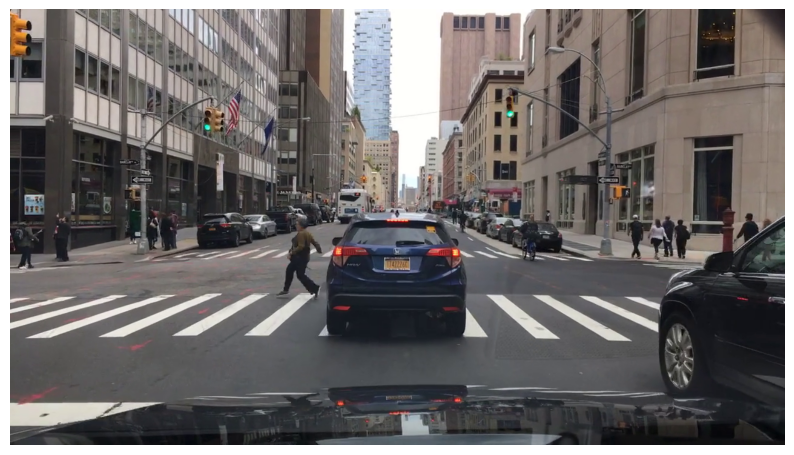
\includegraphics[scale=.4]{images/Figure 1.png}}
\caption{Before Executing YOLO}
\label{fig1}
\end{figure}

\begin{figure}[htbp]
\centerline{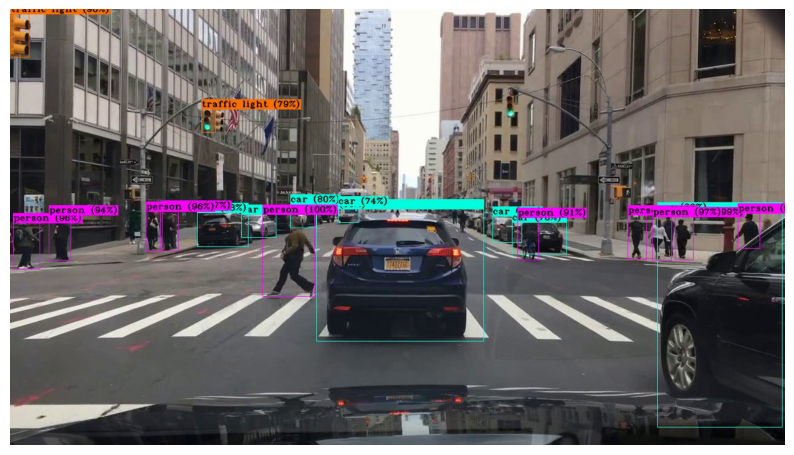
\includegraphics[scale=.4]{images/Figure 2.png}}
\caption{After Executing YOLO}
\label{fig2}
\end{figure}

\subsection{BDD100K}
Datasets are important to machine learning, as they provide the means to train, and test learning models. The Berkeley DeepDrive (BDD100K) 
dataset [6] is critical for training and evaluating machine learning models in computer vision, particularly for autonomous driving
applications. BDD100K consist of a video dataset with 100K videos, and each video having 40 seconds high resolution footage of 
vehicles, people, cyclists, and traffic signs. Conditions include various weather, lighting, and traffic scenarios. This dataset 
is instrumental benchmarking models for real-time object detection in autonomous vehicles.

\section{Methodology}
In this study, we employed a Google Colab [7], a cloud-based platform offering access to CPUs and GPUs, to implement an 
object detection model that uses YOLOv3. Google Colab provides a convenient environment for developing and testing machine learning models, with seamless integration 
of popular libraries and GPU resources. For our experiment, we selected driving videos from the BDD100K dataset, which is well 
suited for evaluating object detection models in autonomous driving scenarios. We opted to use YOLOv3 due to its efficiency, and 
developer documentation. To deploy YOLOv3 for object detection, we utilized OpenCV, a popular Python computer vision library. OpenCV
provides tools for real-time image processing, enabling seamless integration with YOLOv3. The experiments performed in Google Colab, 
used an Intel Xeon CPU @2.2GHz with 39.42 MB cache and an NVIDIA A100-SXM4-40GB GPU. This hardware setup is more than sufficient 
to run YOLOv3 efficiently, enabling real-time object detection on driving videos from the BDD100K dataset.

\section{Results and Analysis}
We evaluated the performance of YOLOv3 on driving videos from the BDD100K dataset. Figures \ref{fig3}  
depict the frames per second (FPS) achieved during model execution for two sample videos. The results show that 
YOLOv3 achieves a high FPS, making it suitable for real-time application like Advanced Driver Assistance Systems (ADAS)
\begin{figure}[htbp]
\centerline{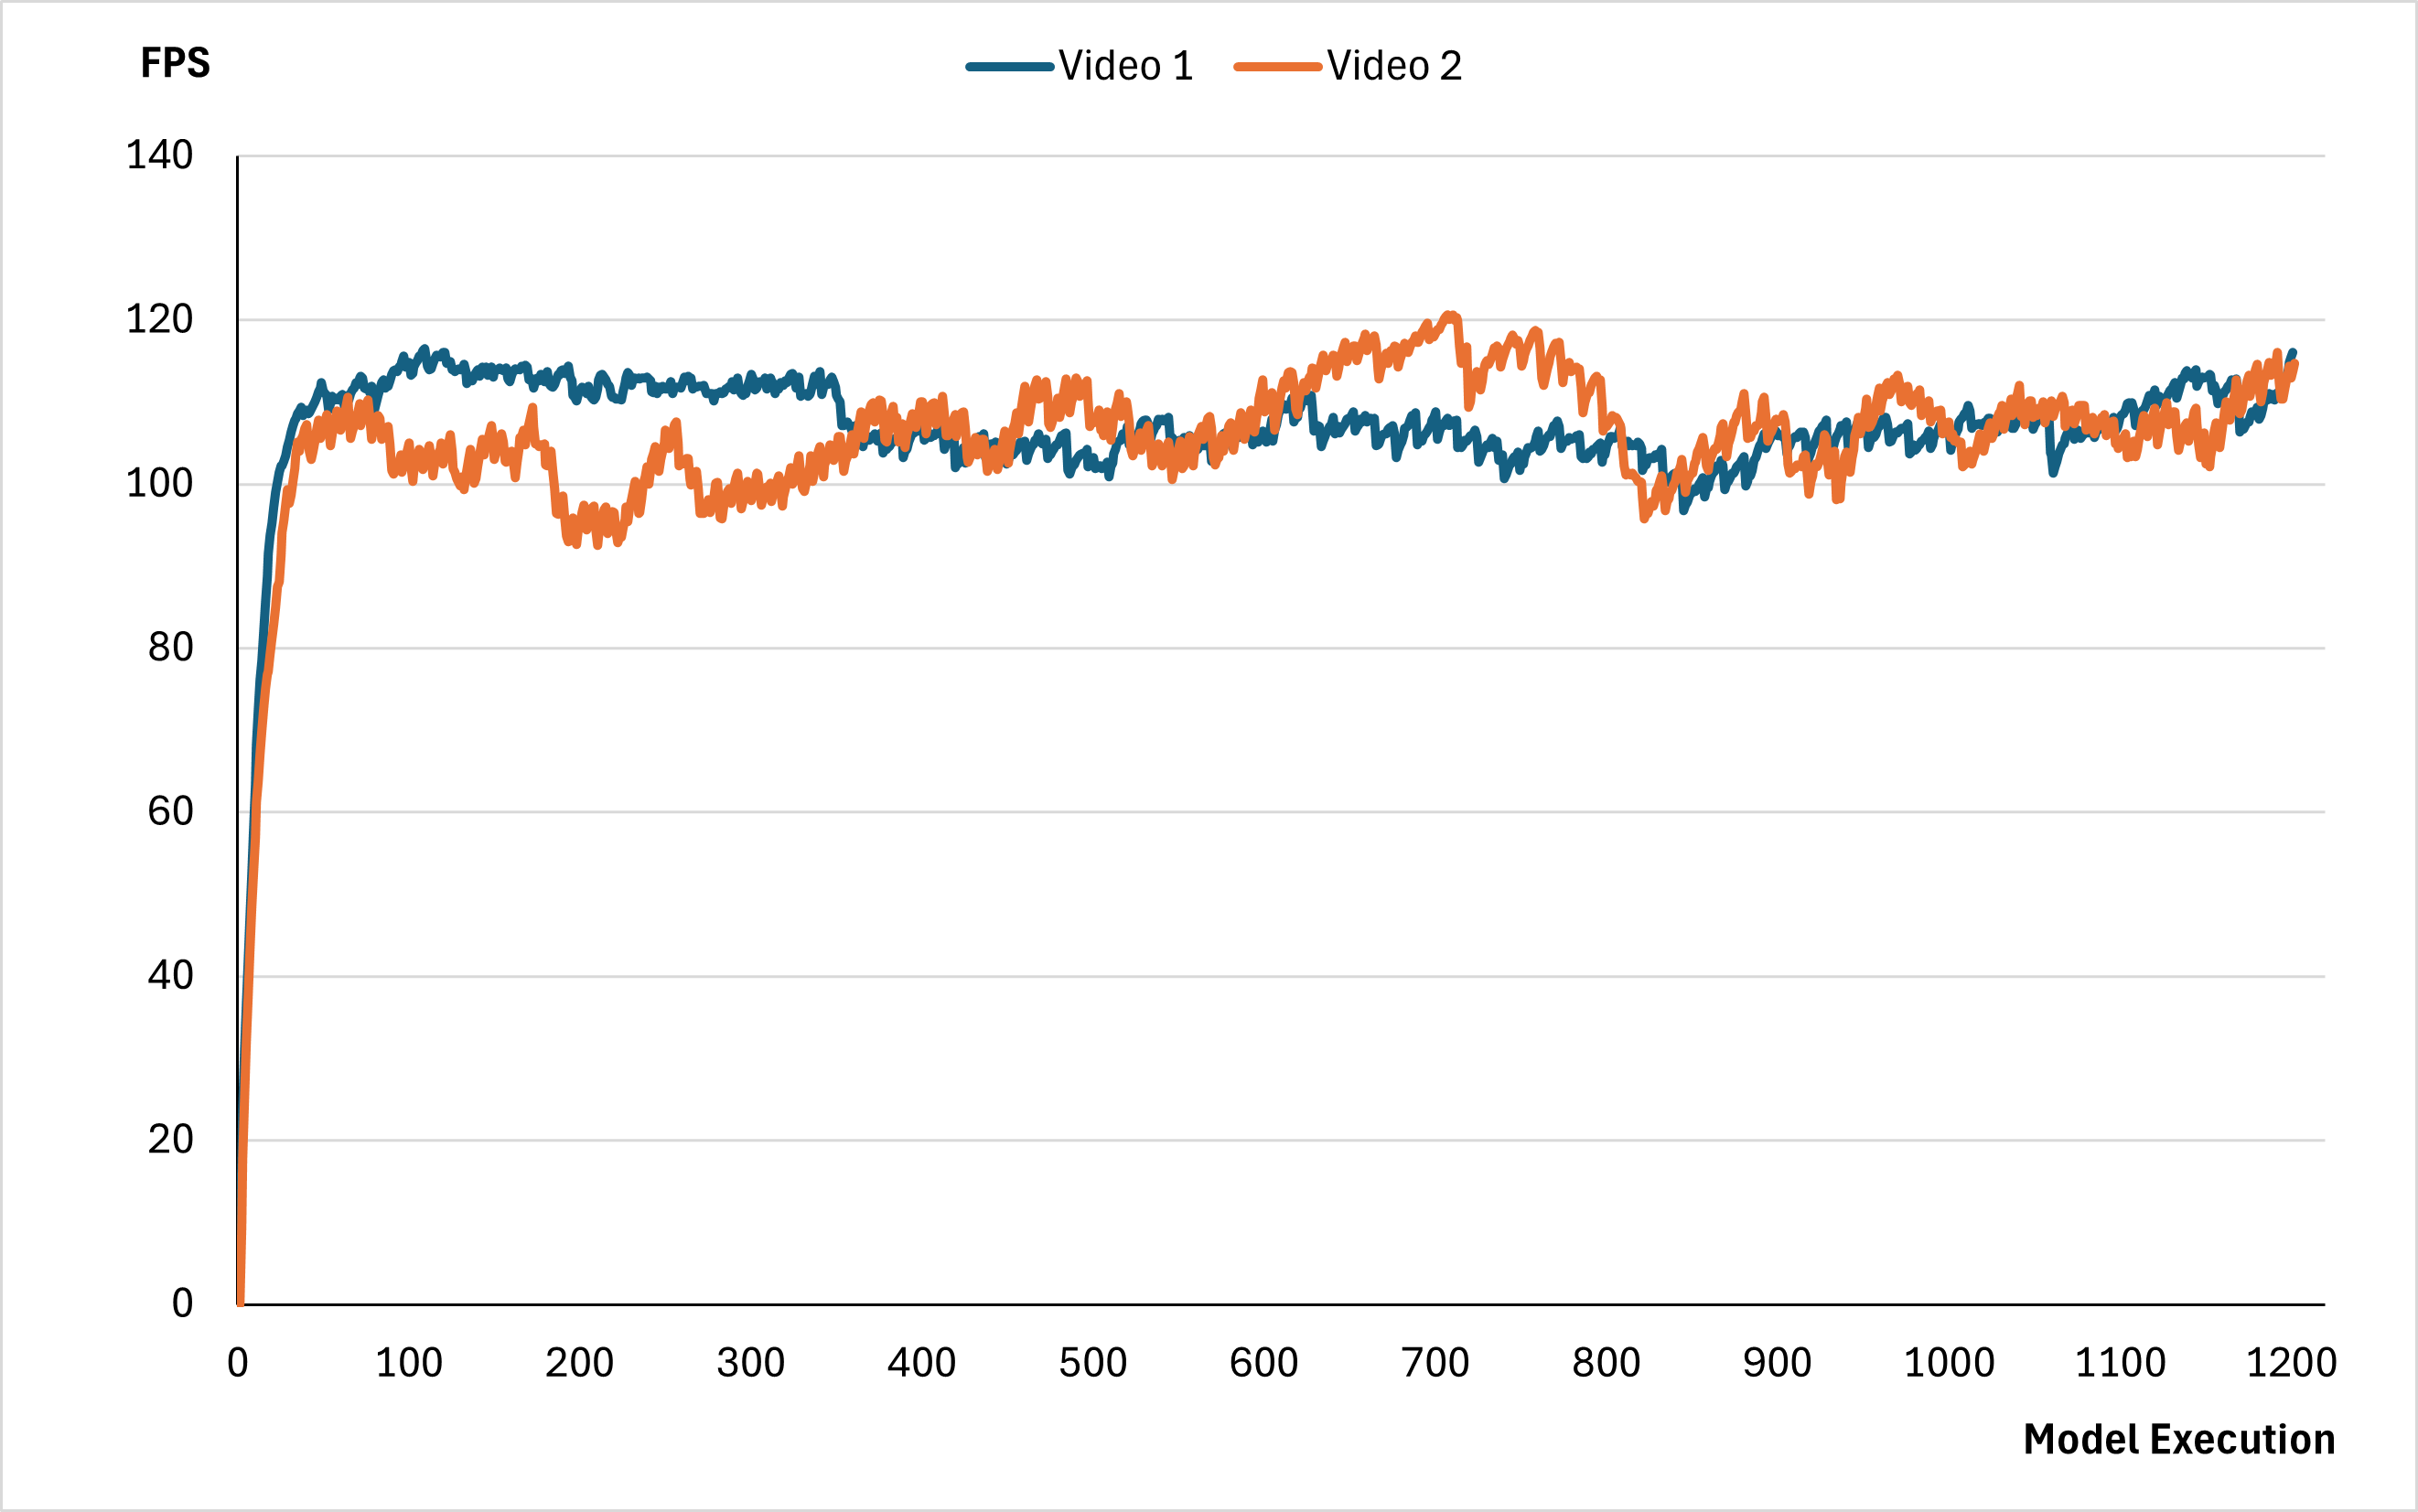
\includegraphics[scale=.4]{images/Figure 3.png}}
\caption{FPS vs. Model Execution of Video 1.}
\label{fig3}
\end{figure}

\section{Discussion and Future Research}
The results indicate YOLOv3 can effectively detect objects in driving scenarios, showing promise for ADAS. However, 
there are opportunities for future research to enhance this growing field further:
\begin{itemize}
    \item \textbf{Exploring YOLO Models:}
    Future work will involve implementing  other YOLO models.
    \item \textbf{Improving Accuracy:}
    Investigate techniques to improve accuracy, especially in challenging conditions [8].
    \item \textbf{Sensor Fusion Integration:}
    Explore methods to integrate YOLO with other sensors such as lidar, and radar.
    \item \textbf{Real-time Systems:}
    Implement YOLO on embedded systems with limited computational resources [9].
\end{itemize}

\section{Conclusion}
In conclusion, our study demonstrates the feasibility of using YOLOv3 for real-time object detection in driving 
scenarios, especially for ADAS applications. YOLOv3 offers a balance between speed and accuracy, making it suitable choice
for enhancing road safety and autonomy in vehicles. 
\begin{thebibliography}{00}
\bibitem{b1}
J. Bian et al., "Machine Learning in Real-Time Internet of Things (IoT) Systems: A Survey," in IEEE Internet of Things Journal, vol. 9, no. 11, pp. 8364-8386, 1 June1, 2022, doi: 10.1109/JIOT.2022.3161050.

\bibitem{b2}
A. Rahimpour, N. Fallahinia, D. Upadhyay and J. Miller, "Deer in the headlights: FIR-based Future Trajectory Prediction in Nighttime Autonomous Driving," 2023 IEEE Intelligent Vehicles Symposium (IV), Anchorage, AK, USA, 2023, pp. 1-6, doi: 10.1109/IV55152.2023.10186756.

\bibitem{b3}
A. Møgelmose, A. Prioletti, M. M. Trivedi, A. Broggi and T. B. Moeslund, "Two-stage part-based pedestrian detection," 2012 15th International IEEE Conference on Intelligent Transportation Systems, Anchorage, AK, USA, 2012, pp. 73-77, doi: 10.1109/ITSC.2012.6338898.

\bibitem{b4}
J. Redmon, S. Divvala, R. Girshick and A. Farhadi, "You Only Look Once: Unified, Real-Time Object Detection," 2016 IEEE Conference on Computer Vision and Pattern Recognition (CVPR), Las Vegas, NV, USA, 2016, pp. 779-788, doi: 10.1109/CVPR.2016.91.

\bibitem{b5}
Y. Yu, S. Yan and X. Hao, "Pedestrian Detection Based on Improved YOLOv3 Network," 2023 IEEE International Conference on Control, Electronics and Computer Technology (ICCECT), Jilin, China, 2023, pp. 297-301, doi: 10.1109/ICCECT57938.2023.10141270.

\bibitem{b6}
F. Yu et al., "BDD100K: A Diverse Driving Dataset for Heterogeneous Multitask Learning," 2020 IEEE/CVF Conference on Computer Vision and Pattern Recognition (CVPR), Seattle, WA, USA, 2020, pp. 2633-2642, doi: 10.1109/CVPR42600.2020.00271.

\bibitem{b7}
Google. (2024). Google Colaboratory. Retrieved May 6, 2024, from https://colab.research.google.com/

\bibitem{b8}
M. Hnewa and H. Radha, "Object Detection Under Rainy Conditions for Autonomous Vehicles: A Review of State-of-the-Art and Emerging Techniques," in IEEE Signal Processing Magazine, vol. 38, no. 1, pp. 53-67, Jan. 2021, doi: 10.1109/MSP.2020.2984801

\bibitem{b9}
V. Shahane, H. Jadhav, M. Sansare and P. Gunjgur, "A Self-Driving Car Platform Using Raspberry Pi and Arduino," 2022 6th International Conference On Computing, Communication, Control And Automation (ICCUBEA, Pune, India, 2022, pp. 1-6, doi: 10.1109/ICCUBEA54992.2022.10010814.

\end{thebibliography}

\end{document}
